\documentclass[11pt,a4paper]{article}
\usepackage[T1]{fontenc}
\usepackage[margin=2.3cm]{geometry}
\usepackage{amsmath,amssymb}
\usepackage{graphicx}
\usepackage[dvipsnames]{xcolor}
\usepackage{enumitem}
\usepackage[colorlinks=true,linkcolor=blue,urlcolor=blue]{hyperref}
\setlength{\parskip}{0.6em}
\setlength{\parindent}{0pt}
\begin{document}

\begin{center}{\LARGE\bfseries openupi}\\[0.4em]{\large Trace a digital payment from tap to bank balance, in three sessions.}\\[0.2em]\small PAN IIT OSS explainer \textbullet{} middle school to higher secondary (levels 2-4)\end{center}

\section*{Why this exists}
Every digital payment is a short conversation between a payer app, a switch and two banks, ending in two numbers changing. This explainer shows the ideas behind it: ledgers, all-or-nothing writes, safe retries and simple fraud checks, using only counting and probability, so you can build it yourself.

\section*{The end goal}
Trace a digital payment from tap to bank balance, and spot where fraud checks sit. The end goal is to trace a digital payment from tap to bank balance and to see where fraud checks sit. It is a toy model that borrows only the ideas of real payment systems; it is not a design for real money and uses no real bank data, networks or protocols.

\section*{How the three sessions build up}
\begin{enumerate}[nosep]
\item \textbf{Session 1: The cast of a payment and its message flow} (Level 1, conceptual interactive model, 60 min).
\item \textbf{Session 2: A ledger, atomic payments and safe retries} (Level 2, mathematical engineering model, 75 min).
\item \textbf{Session 3: A toy payment switch: failures, invariants and fraud rules} (Level 3, simulation and validation, 90 min).
\end{enumerate}

\section{Session 1: The cast of a payment and its message flow}

\subsection*{A. Real-world problem}
You scan a code at a shop, type your PIN, and a moment later both phones say success. Nothing physical moved. So what actually happened, who talked to whom, and where was your money while the screen was spinning? This session is general education about how such systems are organised, not advice about any real app, bank or account, and it uses a simplified picture.

\subsection*{B. Concept and theory}
A payment involves a cast. The payer app and payee app are only windows on phones: they send and show messages and hold no money. Each customer's money is a number in a ledger kept by that customer's bank. A switch in the middle passes messages between apps and banks and tracks the payment on its way. The payer app asks the switch to pay X rupees; the switch asks the payer bank to debit X; the payer bank lowers the payer's ledger number and says so; the switch asks the payee bank to credit X; the payee bank raises the payee's ledger number and says so; and the switch tells both apps. Between the debit and the credit the X rupees are in flight: we count them in a box at the switch so that every rupee always has exactly one home. If the payer's balance is smaller than X, the payer bank declines and nothing moves.

\begin{itemize}[nosep]
\item X: payment amount (rupees)
\item P: payer's ledger balance at the payer bank (rupees)
\item Q: payee's ledger balance at the payee bank (rupees)
\item F: money in flight at the switch (rupees)
\item T: total of all three boxes (rupees)
\item k: step in the message flow (0 to 6) (count)
\end{itemize}

\begin{equation*}
P' = P - X,\qquad Q' = Q + X\qquad (X \le P)
\end{equation*}

\begin{equation*}
T = P + F + Q
\end{equation*}

\begin{equation*}
T_{\text{after}} = T_{\text{before}}\quad\text{(no money is created or lost)}
\end{equation*}

\begin{center}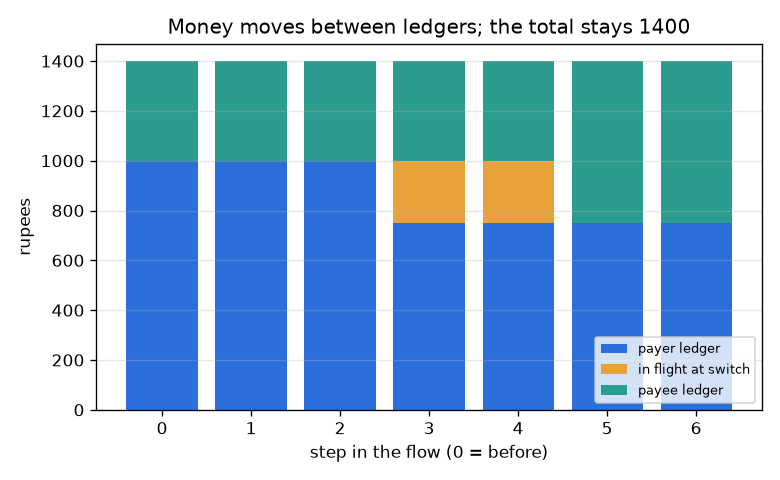
\includegraphics[width=0.85\linewidth]{figures/s01_ledgers_by_step.png}\\\small Payer ledger, in-flight money and payee ledger at each step: the total stays 1400 rupees.\end{center}

\subsection*{E. Worked example}
The payer has Rs 1000 and the payee has Rs 400. The payer pays Rs 250. Find the three numbers after each step and check the total.
\begin{enumerate}[nosep]
\item Before step 3 nothing has moved: payer 1000, in flight 0, payee 400, total 1400.
\item Step 3 (payer bank debits): payer = 1000 - 250 = 750 and in flight = 250. Total = 750 + 250 + 400 = 1400.
\item Step 4 (switch asks payee bank): nothing changes yet.
\item Step 5 (payee bank credits): in flight = 0 and payee = 400 + 250 = 650. Total = 750 + 0 + 650 = 1400.
\item Sanity check: the payer lost 250 and the payee gained 250, so the total did not change.
\end{enumerate}
\textbf{Answer.} After the last message the payer has Rs 750, the payee Rs 650, nothing is in flight, and the total is still Rs 1400.

\subsection*{F. Questions}
\begin{enumerate}[nosep]
\item \textbf{Conceptual.} Why do the payer app and the payee app hold no money, and why do we need the in-flight box at the switch?
\item \textbf{Numerical.} The payer has Rs 2000 and the payee has Rs 150. The payer pays Rs 600. Give the three numbers after step 3 and after step 6, and the total each time.
\item \textbf{Graph and simulation interpretation.} In the stacked-bar figure, at which steps is there an orange in-flight block, and what happens to the total height?
\item \textbf{Design and optimisation challenge.} Design: the switch crashes after step 3 and never sends step 4. The payer has lost Rs 250 and the payee has gained nothing. Describe two sensible ways the system could recover, and what each would have to remember.
\end{enumerate}

\section{Session 2: A ledger, atomic payments and safe retries}

\subsection*{A. Real-world problem}
You tap pay, the screen freezes, so you tap again. Did the shop get paid once or twice? A bank must get this right millions of times a day, even when its software crashes in the middle of a payment. The tools are old and simple: a double-entry ledger, atomic transactions and idempotency. This is general education about how such systems are built, not advice about any real account.

\subsection*{B. Concept and theory}
An entry is (transaction id, account, signed amount): money leaving an account is negative, money arriving is positive. A payment writes two entries with the same transaction id, so its entries sum to zero. We never store a balance on its own: the balance of an account is the sum of its entries. A special account MINT is where money enters the toy world, so even a deposit has two sides, and then the whole ledger always sums to zero and customer money equals money deposited. A transaction is atomic if either both entries are written or neither is; we get that by preparing both entries first and writing them in one step. A request is idempotent if doing it again changes nothing: the ledger remembers the first reply for each transaction id and returns it for any repeat. The order of checks matters: authenticate first, look for a duplicate id before checking the balance (a successful payment lowers the balance, so a retry would otherwise be wrongly declined), then validate the amount and limit, then the accounts, then the balance. Without an id check, n arrivals of a request for X from a balance B0 give min(n, floor(B0 / X)) charges; with it, exactly one charge if 0 \textless{} X \textless{}= B0, otherwise none.

\begin{itemize}[nosep]
\item entry: (transaction id, account, signed amount) (id, name, rupees)
\item B(a): balance of account a (rupees)
\item X: payment amount (rupees)
\item B0: payer's starting balance (1000) (rupees)
\item n: how many times the same request arrives (count)
\item c: number of times the payer is charged (count)
\end{itemize}

\begin{equation*}
B(a)=\sum_{e\,:\,\text{account}(e)=a}\text{amount}(e)
\end{equation*}

\begin{equation*}
\sum_{\text{all entries}}\text{amount}(e)=0\quad\Longrightarrow\quad \sum_{a\neq \text{MINT}}B(a)=\text{money deposited}
\end{equation*}

\begin{equation*}
c_{\text{no id check}}=\min\!\left(n,\left\lfloor \frac{B_0}{X}\right\rfloor\right),\qquad c_{\text{id check}}=1\ \ (0<X\le B_0)
\end{equation*}

\begin{equation*}
B_{\text{payer, after}}=B_0-X\,c
\end{equation*}

\begin{center}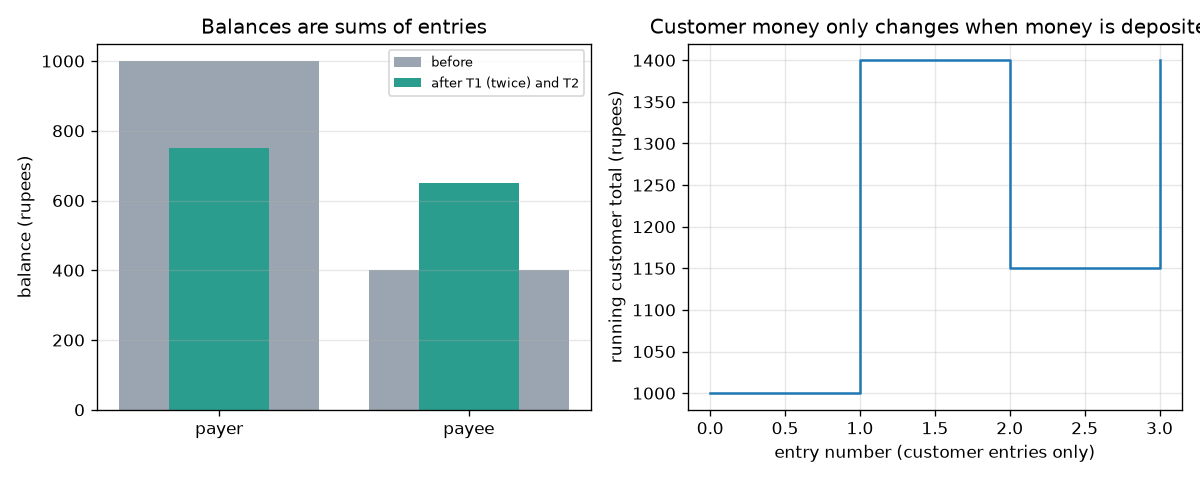
\includegraphics[width=0.85\linewidth]{figures/s02_ledger_balances.png}\\\small Balances before and after, and the running customer total that only changes at deposits.\end{center}

\subsection*{E. Worked example}
Start with payer 1000 and payee 400. Process (T1: pay 250), then (T1 again), then (T2: pay 900). Give the final balances and say what each reply is.
\begin{enumerate}[nosep]
\item T1 is new, authenticated, 250 is within the limit and 1000 \textgreater{}= 250, so it is committed: payer 750, payee 650. Reply: ok.
\item T1 again is a duplicate id, so the saved reply (ok) is returned and nothing is written. The balances stay 750 and 650.
\item T2 asks for 900 but the payer has only 750, so it is declined: insufficient balance. Nothing moves.
\item Check: the entries are two deposits and one payment; every transaction sums to 0, the ledger sums to 0, and payer + payee = 750 + 650 = 1400 = 1000 + 400.
\end{enumerate}
\textbf{Answer.} Payer Rs 750, payee Rs 650, customer total Rs 1400; the replies are ok, ok (replayed) and declined (insufficient balance).

\subsection*{F. Questions}
\begin{enumerate}[nosep]
\item \textbf{Conceptual.} Why is it a problem if a program writes the debit, then crashes before writing the credit? What does writing both entries in one step change?
\item \textbf{Numerical.} The payer has Rs 1000. A request for Rs 300 arrives 5 times. How much is the payer charged in total, and what are both balances, (a) without an id check and (b) with one? The payee starts with Rs 400.
\item \textbf{Graph and simulation interpretation.} In the retries figure (Rs 250 from Rs 1000), what are the payer balances without the id check for 1, 2, 3, 4 and 8 arrivals, and why does the red curve go flat?
\item \textbf{Design and optimisation challenge.} Design: list the checks a bank should run before debiting in a good order, and for each say what goes wrong if it is moved. Assume a per-payment limit of Rs 2000.
\end{enumerate}

\section{Session 3: A toy payment switch: failures, invariants and fraud rules}

\subsection*{A. Real-world problem}
Real payment systems must stay correct when messages are lost, when people tap twice, and when someone who is not the owner tries to pay. Today you build a toy in-memory payment switch with accounts, a transaction log, a safely stored PIN, an idempotency key and simple fraud rules, stress it with invented trouble, and check that nobody is charged twice. It is a toy that borrows only the ideas: there is no networking, no real bank, no real UPI protocol and no real data. The fraud part is about defence: where checks sit and how well they work. General education only, not advice about any real account.

\subsection*{B. Concept and theory}
PIN safety: never store a PIN. Store hash\_pin(PIN, salt), where the salt is random and different for each account and the hash (PBKDF2 with SHA-256, many repetitions) is slow to compute on purpose. To check an attempt, hash it with the stored salt and compare using a constant-time comparison (hmac.compare\_digest), which does not reveal through timing where the first difference is. A 4-digit PIN has only 10000 values, so hashing alone cannot protect a stolen hash from being guessed; real systems also lock after a few wrong attempts (we lock after 3) and keep checks in secured hardware. Failure injection: each attempt is lost before reaching the switch with probability p\_req, or processed with its reply lost with probability p\_rep. The phone retries with the same transaction id up to k times. With a = 1 - p\_req and s = a(1 - p\_rep), the expected number of charges per payment without an id check is a(1 - (1 - s)\textasciicircum{}k) / s, and with an id check it is 1 - p\_req\textasciicircum{}k (charged once if it ever arrives). Invariants: (1) all entries sum to zero and customer balances sum to the money put in; (2) no balance is negative; (3) each transaction id has at most one debit. A double charge keeps (1) and (2) true, which is why (3) is separate. Fraud rules run before the commit: velocity (more than V completed payments in 10 minutes), unusual amount (more than M times the account's median past amount, once there is history) and new payee (a payee not paid before, with amount at least 1000). A flagged payment is held until the owner confirms. The false positive rate is the share of ordinary payments flagged; the false negative rate is the share of fraud payments not flagged.

\begin{itemize}[nosep]
\item p\_req: chance an attempt is lost before the switch (probability (0 to 1))
\item p\_rep: chance a processed attempt's reply is lost (probability (0 to 1))
\item k: maximum attempts by the phone (count)
\item a, s: a = 1 - p\_req; s = a(1 - p\_rep) (probability)
\item E: expected charges per payment (count)
\item V, M: velocity limit (payments per 10 minutes) and amount multiple (count, no unit)
\item FPR, FNR: false positive rate, false negative rate (fraction or percent)
\end{itemize}

\begin{equation*}
E[\text{charges, no key}]=\frac{a\,\bigl(1-(1-s)^{k}\bigr)}{s},\qquad a=1-p_{\text{req}},\ \ s=a\,(1-p_{\text{rep}})
\end{equation*}

\begin{equation*}
E[\text{charges, with key}]=1-p_{\text{req}}^{\,k}
\end{equation*}

\begin{equation*}
\mathrm{FPR}=\frac{FP}{FP+TN},\qquad \mathrm{FNR}=\frac{FN}{FN+TP}
\end{equation*}

\begin{equation*}
\text{invariants:}\ \ \sum_{e}\text{amount}(e)=0,\quad B(a)\ge 0,\quad \#\{\text{debits of one id}\}\le 1
\end{equation*}

\begin{center}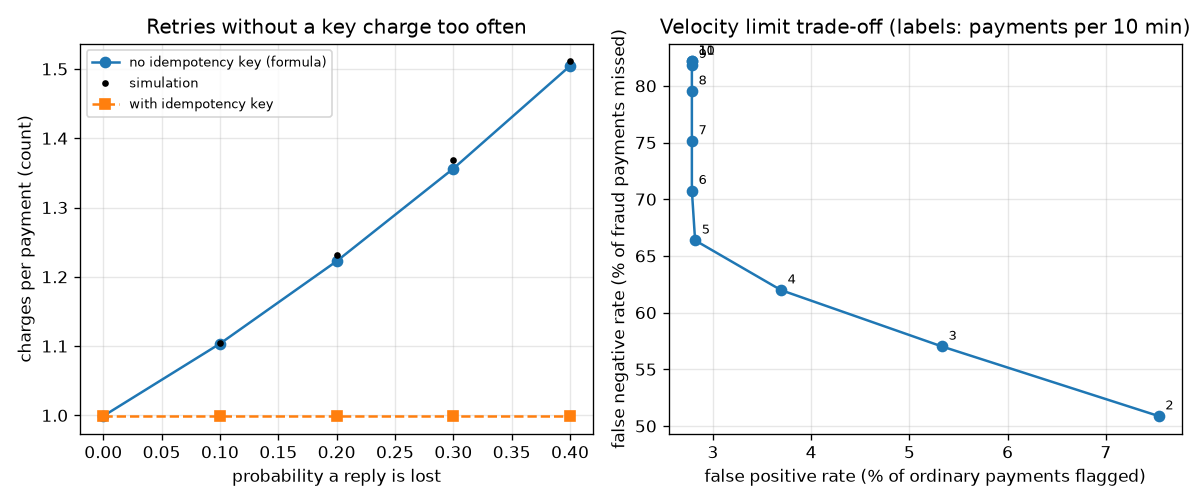
\includegraphics[width=0.85\linewidth]{figures/s03_failures_and_fraud.png}\\\small Left: expected charges per payment against reply loss (formula, simulation, with key). Right: velocity-limit trade-off between false positives and false negatives.\end{center}

\subsection*{E. Worked example}
A test set has 1000 ordinary payments and 50 fraud payments. The rules flag 30 ordinary payments and 40 fraud payments. Find the false positive rate and the false negative rate and say what each means.
\begin{enumerate}[nosep]
\item Ordinary payments: flagged = 30 (false positives, FP = 30), not flagged = 970 (true negatives, TN = 970).
\item FPR = FP / (FP + TN) = 30 / 1000 = 0.03, that is 3 percent of ordinary payments were wrongly flagged.
\item Fraud payments: flagged = 40 (true positives, TP = 40), not flagged = 10 (false negatives, FN = 10).
\item FNR = FN / (FN + TP) = 10 / 50 = 0.20, that is 20 percent of fraud payments were missed.
\item Sanity check: 30 + 970 = 1000 and 40 + 10 = 50, so every payment is counted once. On the lesson's seeded data the default rules give FPR 2.818 percent and FNR 66.374 percent, much worse on misses because slow, small attacks hide among ordinary payments.
\end{enumerate}
\textbf{Answer.} FPR = 3 percent and FNR = 20 percent. Annoyed customers: 3 in 100 ordinary payments; missed fraud: 1 in 5 fraud payments.

\subsection*{F. Questions}
\begin{enumerate}[nosep]
\item \textbf{Conceptual.} Why do we store a salted hash of a PIN instead of the PIN, and why compare with compare\_digest instead of ==? Why is hashing still not enough for a 4-digit PIN?
\item \textbf{Numerical.} With p\_req = 0.1, p\_rep = 0.2 and k = 3, compute a, s, the expected charges per payment without a key and with a key, and the expected extra charges per 100 payments.
\item \textbf{Graph and simulation interpretation.} In the right-hand panel of the first figure, what happens to FPR and FNR when the velocity limit V changes from 5 to 3, and which kind of mistake does each setting prefer?
\item \textbf{Design and optimisation challenge.} Design: you may annoy at most 4 percent of ordinary payments. Choose the velocity limit V from the sweep (V = 2 to 11 gives FPR 7.54, 5.33, 3.69, 2.82, 2.79, 2.79, ...) and then say what else you would add to catch slow, small attacks and what you would use to cap the damage if a burst gets through.
\end{enumerate}

\section{Real-world mini-project}
\textbf{Add a daily limit and stop a rapid-fire burst.} Fraud rules can miss things, so a bank also caps the damage. In Session 3 the toy \texttt{Switch} has no daily limit: \texttt{rapid\_fire\_test} sends 40 payments of Rs 900 and all 40 succeed, so Rs 36000 leaves one account. Add a \texttt{daily\_limit} option to \texttt{Switch} (a day is 1440 simulated minutes, counted from \texttt{now}), refuse a payment that would take the day's total above the limit, and record the reason \texttt{daily limit} in the log. Use a limit of Rs 5000.

\section{The path ahead}
\begin{enumerate}[nosep]
\item \textbf{Session 4: Reconcile three ledgers at the end of the day.} A version of the switch with three separate ledgers (payer bank, switch, payee bank), bank timeouts injected, and a reconciliation step that repairs mismatches.
\item \textbf{Session 5: Catch the slow attack.} A better scoring function than the three fixed rules, judged on the same seeded synthetic data.
\item \textbf{Session 6: Lockout that recovers.} A lockout that expires after 30 simulated minutes and a counter that is kept per account and per day.
\item \textbf{Session 7: Survive a crash: a write-ahead log.} A switch that appends each payment to a log file first and rebuilds all balances and its id memory by replaying it.
\item \textbf{Session 8: Two payments at once.} A threaded test harness and per-account locking in the switch.
\end{enumerate}

\section{Answers and hints}

\subsection*{Session 1}
\begin{enumerate}[nosep]
\item \textbf{Conceptual.} Hint: Where do the ledger numbers live, and where is the money between steps 3 and 5? Solution: The apps are only windows that send and show messages. The ledger numbers live at the banks. Between the debit (step 3) and the credit (step 5) the payer's ledger is already lower but the payee's is not yet higher. Counting the money in an in-flight box gives every rupee exactly one home at every moment, so the total stays the same and we can check it.
\item \textbf{Numerical.} Hint: Step 3 moves the amount into flight; step 5 moves it into the payee ledger. Solution: After step 3: payer 2000 - 600 = 1400, in flight 600, payee 150, total 2150. After step 6: payer 1400, in flight 0, payee 150 + 600 = 750, total 1400 + 0 + 750 = 2150. Units: rupees. The total is the same, as it must be.
\item \textbf{Graph and simulation interpretation.} Hint: Find the steps where the debit has happened but the credit has not. Solution: The orange block exists after steps 3 and 4 only: the debit has happened, the credit has not. The total height is 1400 rupees at every step, because the blue block loses exactly what the orange block gains, and the orange block loses exactly what the green block gains.
\item \textbf{Design and optimisation challenge.} Hint: Either finish the payment or undo it. What record would let you decide? Solution: Option 1, complete: the switch (or a restart procedure) re-sends the credit to the payee bank using the same transaction id, so a repeated credit cannot be applied twice. Option 2, reverse: the payer bank credits Rs 250 back to the payer and records the payment as failed. Either way the system must durably remember the transaction id, the amount, both accounts and how far it got. Trade-off: completing is better for the shop but needs the payee bank to be reachable; reversing is simple but the customer must try again. Session 2 shows how a ledger makes this all-or-nothing.
\end{enumerate}

\subsection*{Session 2}
\begin{enumerate}[nosep]
\item \textbf{Conceptual.} Hint: Add up all the entries after the crash. Solution: After the crash the ledger holds a debit with no matching credit: the entries no longer sum to zero and customer money has dropped by the amount (in the lesson, 250 rupees vanish). If both entries are prepared first and written in one step, a crash before the write leaves the ledger as it was and a crash after leaves a complete payment. Either way the ledger still sums to zero.
\item \textbf{Numerical.} Hint: Without the check, c = min(n, floor(B0 / X)). Solution: (a) floor(1000 / 300) = 3, so c = min(5, 3) = 3 charges: 900 rupees. Payer 1000 - 900 = 100, payee 400 + 900 = 1300, total 1400. (b) One charge: payer 700, payee 700, total 1400. Sanity check: the totals agree, and the balance never went negative because the 4th charge would have needed 1200 \textgreater{} 1000.
\item \textbf{Graph and simulation interpretation.} Hint: Charges are min(n, 4) because floor(1000 / 250) = 4. Solution: 1 arrival: 750; 2: 500; 3: 250; 4: 0; 8: 0. The curve goes flat at 0 because the balance check stops further debits once the money is gone. The flat part is not a safe outcome: the payer has paid four times for one purchase. The green curve stays at 750.
\item \textbf{Design and optimisation challenge.} Hint: Think about strangers, retries of a payment that already happened, and nonsense amounts. Solution: Order: 1 authenticate (otherwise strangers learn about accounts and can probe them); 2 duplicate id (before the balance check, or a retry of a successful 900 payment from 1000 is wrongly declined for 'insufficient balance' because the balance is now 100); 3 amount valid and within the Rs 2000 limit (cheap, blocks nonsense such as 0, negative or fractional amounts); 4 payer is not the payee; 5 sufficient balance. Then commit both entries atomically. Trade-off: every extra check costs time and may block honest users, so limits should be set with real usage in mind. Assumption: one ledger, one request at a time.
\end{enumerate}

\subsection*{Session 3}
\begin{enumerate}[nosep]
\item \textbf{Conceptual.} Hint: Think about a stolen database, two people with the same PIN, and how many 4-digit PINs exist. Solution: If the database is stolen, plain PINs are immediately usable; hashes must be guessed. The salt makes the same PIN give different hashes, so one precomputed table does not work for all accounts. compare\_digest takes the same time wherever the bytes differ, so timing does not leak how many leading bytes were right. There are only 10000 four-digit PINs, so if a hash and salt leak, all can be tried quickly; real systems add lockout after a few wrong attempts and keep PIN checks in secured hardware.
\item \textbf{Numerical.} Hint: a = 0.9, s = 0.9 x 0.8. Use E = a(1 - (1 - s)\textasciicircum{}k)/s and 1 - p\_req\textasciicircum{}k. Solution: a = 0.9 and s = 0.72. (1 - s)\textasciicircum{}3 = 0.28\textasciicircum{}3 = 0.021952, so E = 0.9 x (1 - 0.021952) / 0.72 = 0.9 x 0.978048 / 0.72 = 1.2226. With a key: 1 - 0.1\textasciicircum{}3 = 0.999. Extra = 1.2226 - 0.999 = 0.2236 per payment, about 22.4 per 100 payments. This matches the simulated value 1.2233 in the lesson. Units: charges per payment (a count).
\item \textbf{Graph and simulation interpretation.} Hint: Read the points labelled 5 and 3. Lower V means a stricter rule. Solution: At V = 5: FPR 2.82 percent, FNR 66.4 percent. At V = 3: FPR 5.33 percent, FNR 57.0 percent. The stricter rule flags more ordinary payments (more annoyed customers) and misses fewer fraud payments. Neither is right in general: it depends on the cost of a missed fraud payment against the cost of an annoyed customer. The curve also shows that the velocity limit alone cannot push FNR below about 50 percent here, because it cannot see one large payment or a slow trickle.
\item \textbf{Design and optimisation challenge.} Hint: Find the strictest V with FPR at most 4 percent, then think about other signals and a hard cap. Solution: V = 4 is the strictest limit with FPR 3.69 percent (V = 3 gives 5.33 percent, over budget); its FNR is 62.0 percent. The sweep shows the velocity rule cannot catch slow attacks, so add rules on other signals (for example a lower new-payee amount, a per-customer baseline of typical amounts, a device or location check), accepting more false positives, and measure them with the same synthetic data. To cap the damage if fraud gets through, add a daily limit per account (the mini-project): with a limit of Rs 5000 a burst of Rs 900 payments can take at most 5 x 900 = Rs 4500. Trade-off: every limit also inconveniences honest customers who have a large legitimate need that day, so offer a confirmed way to raise it. Assumption: the synthetic mix of attacks.
\end{enumerate}

\section{How to join}
Read \texttt{CONTRIBUTING.md} in the repository, then pick an issue labelled \texttt{good first issue}. Repository: \url{https://github.com/KrunalPanchal1995/openupi}

\end{document}
